\chapter{Design}

In order to validate the model, a device must be designed, built and tested. 

\section{Selection of design parameters}
There are many parameters to consider when designing LIMs, such as gear ratios, lengths, and wheel size. Optimising the design is beyond the scope of this project, but the device does need to work to the extent that it can be used to validate the model. Initially, this project intended to use the early versions of the model to inform the design process. However, as the model was not yet validated, significantly changing key parameters could easily result in a device that is unable to climb stairs at all. Previous projects were able to show inconsistent success. Of the previous projects, Powrie's design was the latest and most informed, and is used as a starting point for this project. Powrie's report specifies the dimensions and gear ratios for the LIMs used in this project.\\

\section{Body design}
The body of the device is the central part that contains the motors and any peripheral devices.
Powrie's design for the body includes a camera, batteries, and extra gearing to increase the torque of his motor. These components are superfluous for the objectives of this project, and are not included in the design. Additionally, the body in Powrie's design protrudes forward significantly beyond the axle of the LIMs. This is done to allow for gearing of the axial motors used in the design, but previous students have found that this protrusion causes the body to collide with the step when climbing, which can result in failure to climb the step. This project uses DC motors with worm gearbox outputs, allowing the motor to be placed at a right angle to the axis. This eliminates the need for significant forward protrusion or additional gearing, and simplifies the construction process. Figures \ref{fig:Powrie-internals} and \ref{fig:internals} shows the body of Powrie's design and this project's design respectively.
\begin{figure}
	\centering
	\begin{subfigure}{.5\textwidth}
		\centering
		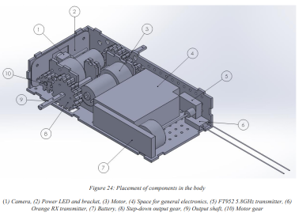
\includegraphics[width=.9\linewidth]{Powrie-internals}
		\caption{Powrie's design of the body.}
		\label{fig:Powrie-internals}
	\end{subfigure}%
	\begin{subfigure}{.5\textwidth}
		\centering
		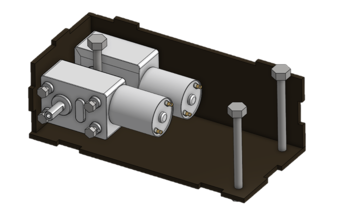
\includegraphics[width=.9\linewidth]{internals}
		\caption{This project's design of the body.}
		\label{fig:internals}
	\end{subfigure}
	\caption{Body design comparison.}
	\label{fig:bodies}
\end{figure}

\section{Motor selection}
Brushed DC motors often include a gearbox to increase the torque of the output at the cost of speed. For this design, the output shaft must be at a right angle to the motor, which is typically done with a worm gearbox. The most readily available motors that meet these requirements are the JGY-370 12V DC worm gear motors, which come with a range of gear ratios. Initially, the 40 RPM model was selected as it provides similar torque to the EGB-380S with added gearing that Powrie used, however initial tests indicated that additional torque was needed for consistent climbing, so the 6 RPM model was used instead.\\
Additionally, these motors have a self-locking gearbox, which improves the controllability of the device, as shutting off the motors will cause the gearbox to lock and the device to stop moving, rather than allowing the device to fall backwards down the steps.

\section{Control circuits and code}
In order to validate the model, the torque of the motors must be variable and reversible. This project uses a L298n H-bridge controlled by an STM32-F303RE Nucleo board to drive the motors. Two potentiometer sliders are used to control the torque of the two motors independently. The sliders are set up as voltage dividers and connected to the ADC channels of the STM32 microcontroller. The microcontroller sends a direction and PWM signal for each motor to the L298n H-bridge, which controls the motor using PWM. The circuit diagram for this set-up is shown in Figure \ref{fig:circuit-diagram}.

\begin{figure}[!h]
	\centering
	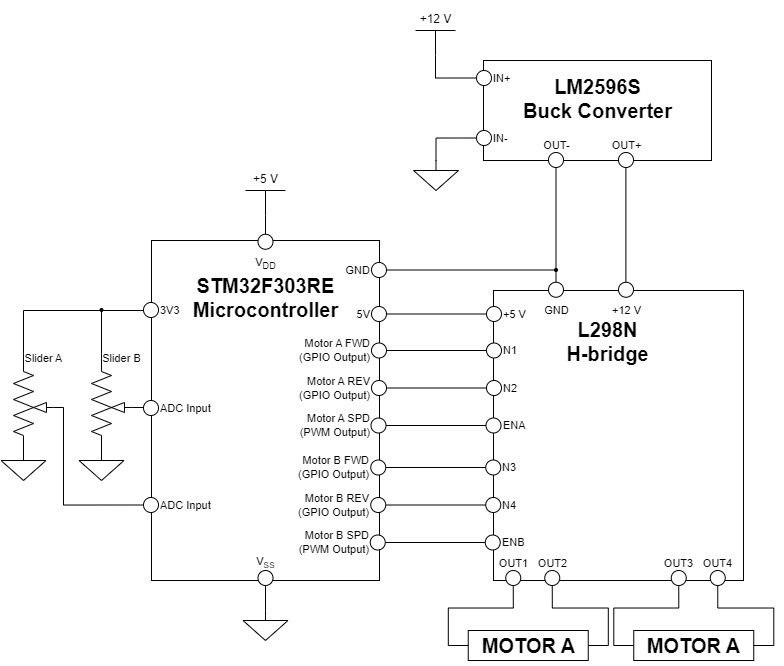
\includegraphics[width=0.8\textwidth]{circuit-diagram}
	\caption{Control system circuit diagram.}
	\label{fig:circuit-diagram}
\end{figure}

The microcontroller is programmed to power off the motors when the sliders are centred, move the motors forward when the sliders are pushed forward, and move the motors in reverse when the sliders are pulled back. The PWM duty cycle is scaled such that when the ADC values are in the centre 20\% of their range, the PWM duty cycle is set to 0\%. When the ADC values are within the top or bottom 5\% of their range, the duty cycle is 100\%. The flow diagram for this code is shown in Figure \ref{fig:controller-flowchart}.

\begin{figure}[!h]
	\centering
	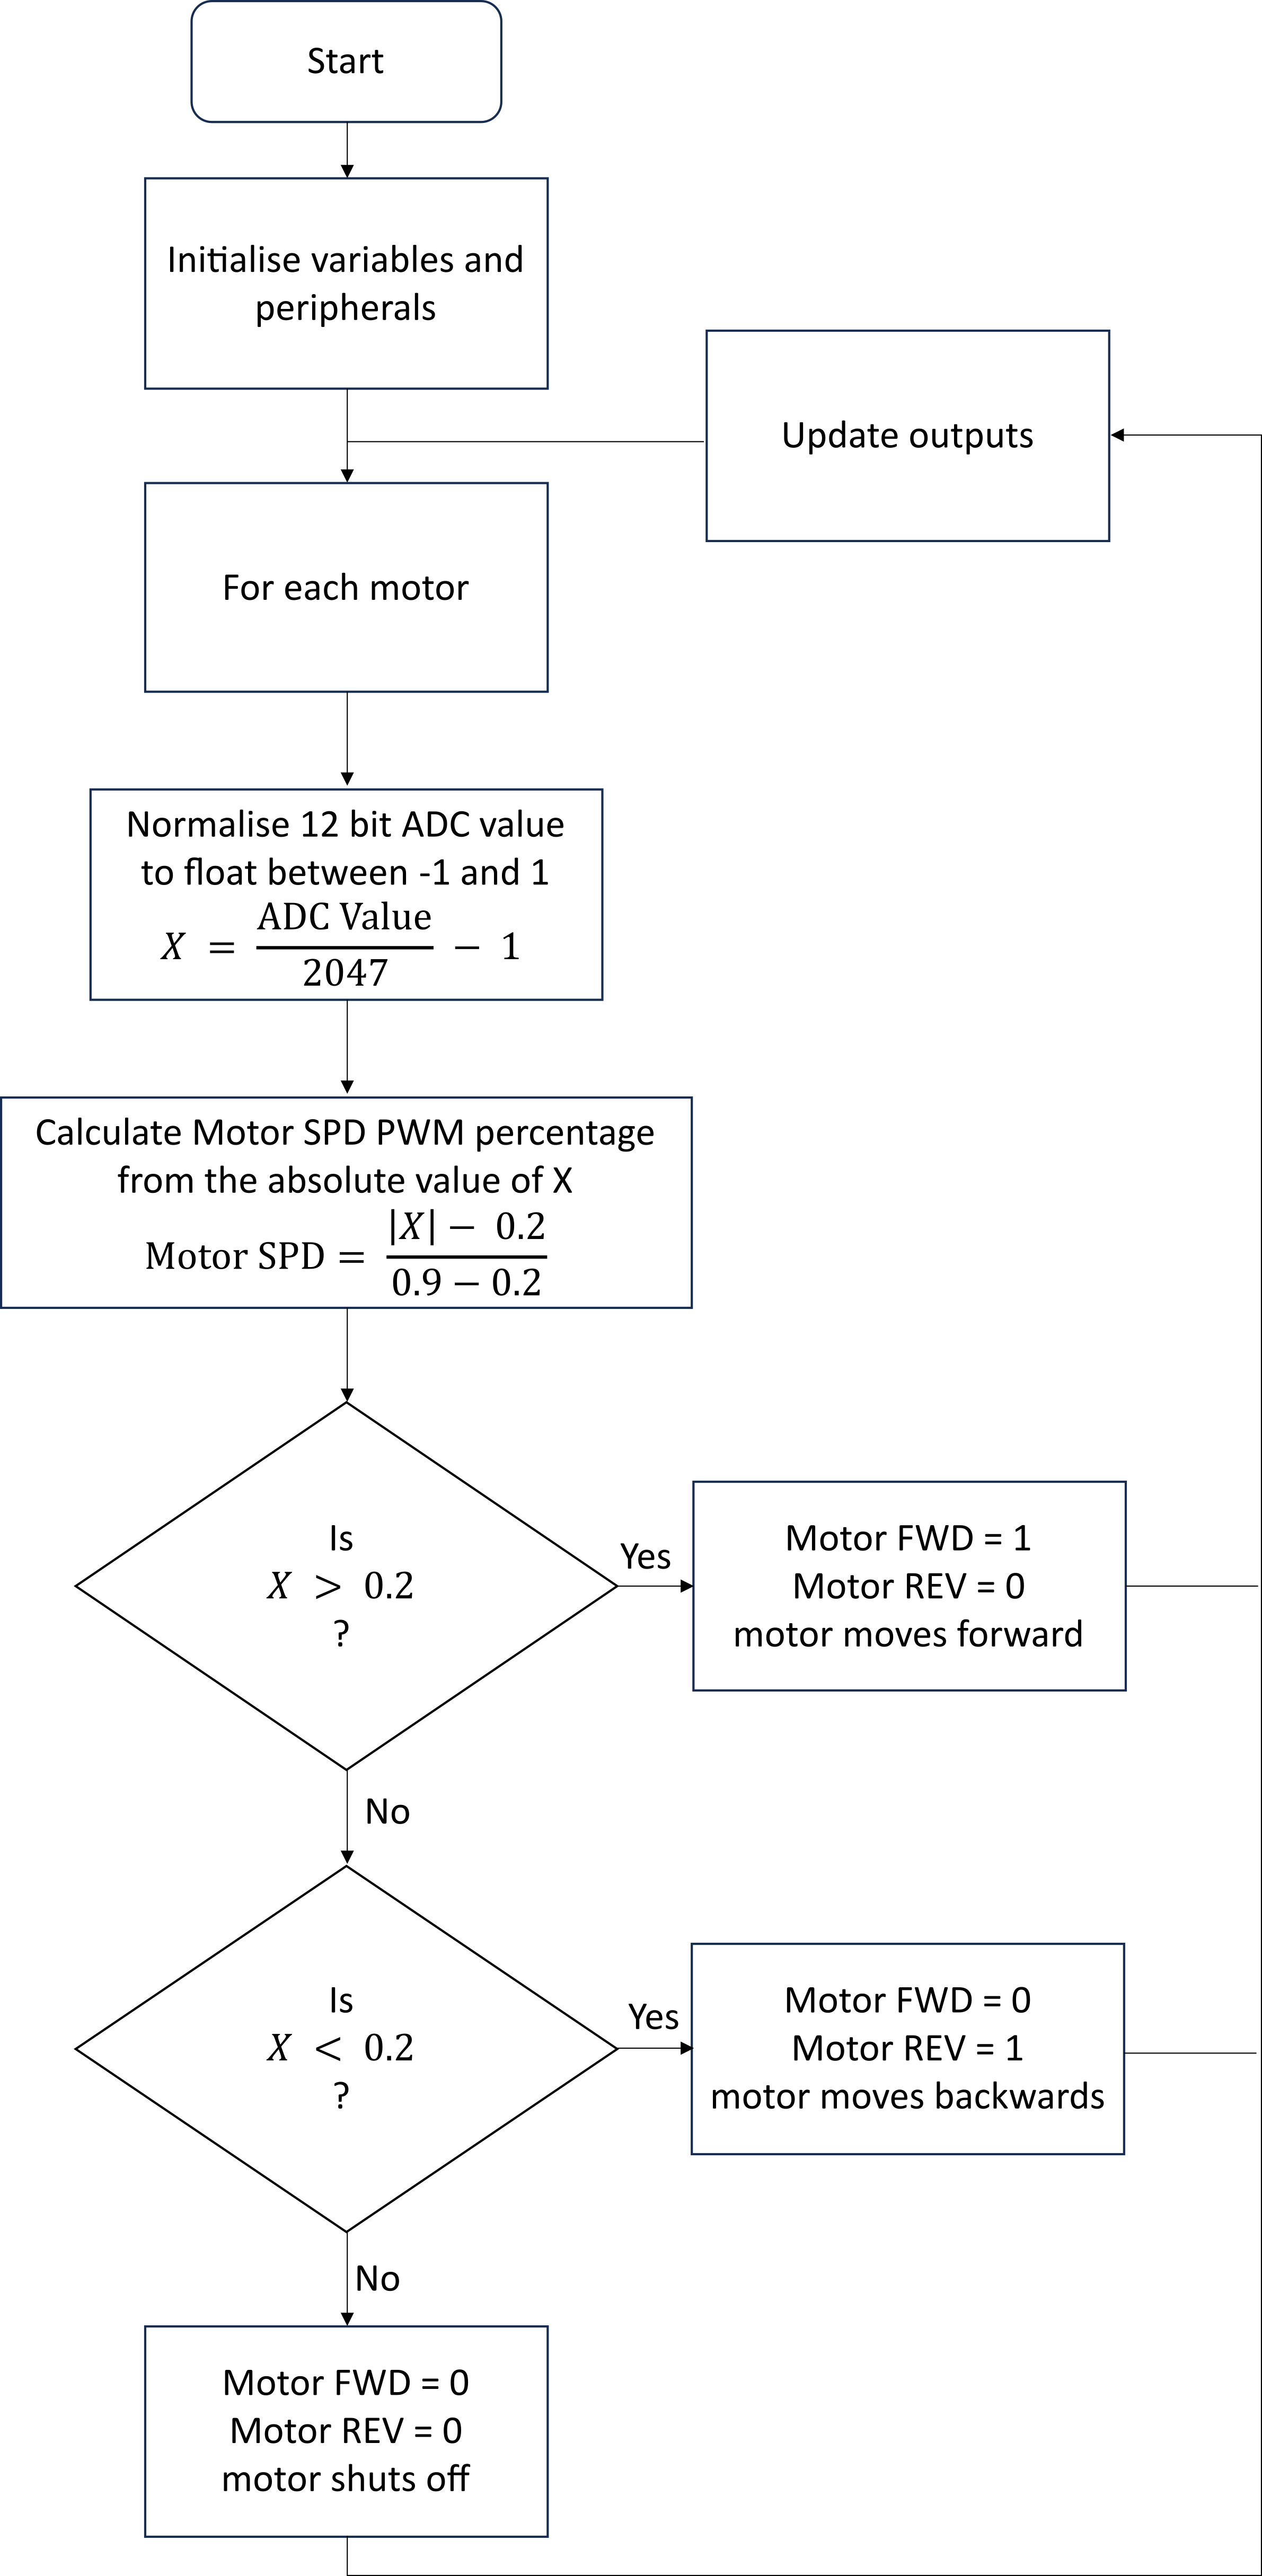
\includegraphics[height=0.8\textheight]{controller-flowchart}
	\caption{Microcontroller code flowchart.}
	\label{fig:controller-flowchart}
\end{figure}

Initial tests showed that PWM duty cycle is not proportional to torque output on the motors. Instead, even at low duty cycles, the motors can lift a large load, they just do so slowly. This is likely because the self-locking gearbox prevents the axle from ever falling backwards. Consider a DC motor lifting a lever as seen in Figure \ref{fig:lever}. 

\begin{wrapfigure}{r}{0.35\textwidth}
	\centering
	\includegraphics[width=0.35\textwidth]{FBDs/lever}
	\caption{Lever example.}
	\label{fig:lever}
\end{wrapfigure}

Typically, when the PWM signal is on, the motor outputs full torque and moves forward, then when the PWM signal is off the motor outputs no torque and falls backwards. The PWM frequency is typically high enough that the human eye sees this as a smooth motion. However, because of the self-locking gearbox, the axle will lock when the PWM signal is off rather than moving backwards, resulting in an overall forward motion even at low duty cycles. This is quite useful for controlling the motors as the speed of the motors is proportional to the PWM duty cycle regardless of the load it must lift.\\

However, for the validation of the model, the motor torque should be variable and measurable. Brushed DC motor torque is proportional to the current running through it, and the current reduces as the speed of the motor increases. The speed of the motor is also proportional to the terminal voltage. The approximate characteristics of a DC motor are given in Figure \ref{fig:torque-speed}. 
\begin{figure}[!h]
	\centering
	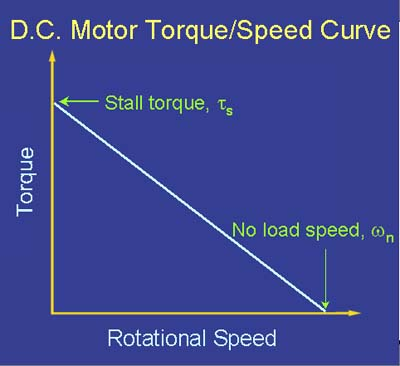
\includegraphics[width=0.35\textwidth]{plots/colorTS1}
	\caption{Torque speed plot of a typical DC motor \citep{Page-1999}.}
	\label{fig:torque-speed}
\end{figure}

\noindent The equation describing the torque of a DC motor in relation to motor voltage and speed is then,
\begin{equation}
	T = T_\mathrm{Rated-stall}(\frac{V_\mathrm{Terminal}}{V_\mathrm{Rated}}-\frac{\omega}{\omega_\mathrm{Rated-no-load}})
\end{equation}
where $T$ is the output torque, $T_\mathrm{Rated-stall}$ is the stalling torque at the rated voltage, $V_\mathrm{Terminal}$ is the supply voltage across the motor terminals, $V_\mathrm{Rated}$ is the motor's rated supply voltage, $\omega$ is the rotational speed of the output shaft, and $\omega_\mathrm{Rated-no-load}$ is the speed of the output shaft when no load is placed on it at the rated voltage.\\

\noindent To solve for the stalling torque, $\omega$ is set to $0$. This gives the relation,
\begin{equation}
	T_\mathrm{Stall} = T_\mathrm{Rated-stall}\frac{V_\mathrm{Terminal}}{V_\mathrm{Rated}}
\end{equation}
%??? Move to literature review?
In order to vary the stall torque of the device, the terminal voltage must be varied. For this purpose, an LM2596S buck converter is used to vary the supply voltage.

\section{Construction and testing}\label{sec:construction}

\begin{wrapfigure}{r}{0.35\textwidth}
	\centering
	\includegraphics[width=0.35\textwidth]{device}
	\caption{Built device.}
	\label{fig:device}
\end{wrapfigure}

To build the device, the parts were laser cut from Medium Density Fibreboard (MDF) and Acrylic. The outer surface of wheels is coated with Patex, a rubbery adhesive which is left to dry, increasing the grip of the wheels. The assembly is relatively straightforward, however it was found that the laser cut gears did not mesh well, causing them to get stuck. To address this, the teeth of the gears were filed down until they could mesh easily. This has the disadvantage of increasing kickback on the gears. However, this has little impact on performance as for all stages of motion, the gears are engaged in one direction only. The device is shown in Figure \ref{fig:device}.\\


Initial tests show that the device is capable of climbing up two steps sequentially, which is more than any previous project achieved. This relative success can be attributed to the shorter forward protrusion of the body and possibly a higher grip on the surface of the wheels. However, the device struggled to climb a third step, this is because climbing the third step involves Stage 4 motion, which requires significantly higher torque than the previous stages. To address this, the body of the device was rebuilt using a JGY-370 gearbox motor which is geared for a higher torque. \\
After this change, the device was able to consistently climb many sequential steps, and the lower speed due to the higher gear ratio made the device easier to control during the climbing motion. Figure \ref{fig:device-climbing} shows the device climbing a flight of stairs. Initial tests also show that by applying a forward torque to one LIM and a reverse torque to the other, the device is capable of turning on the spot. However this motion is inconsistent as the LIMs can start to lift, at which point the turning stops.
\begin{figure}[!ht]
	\centering
	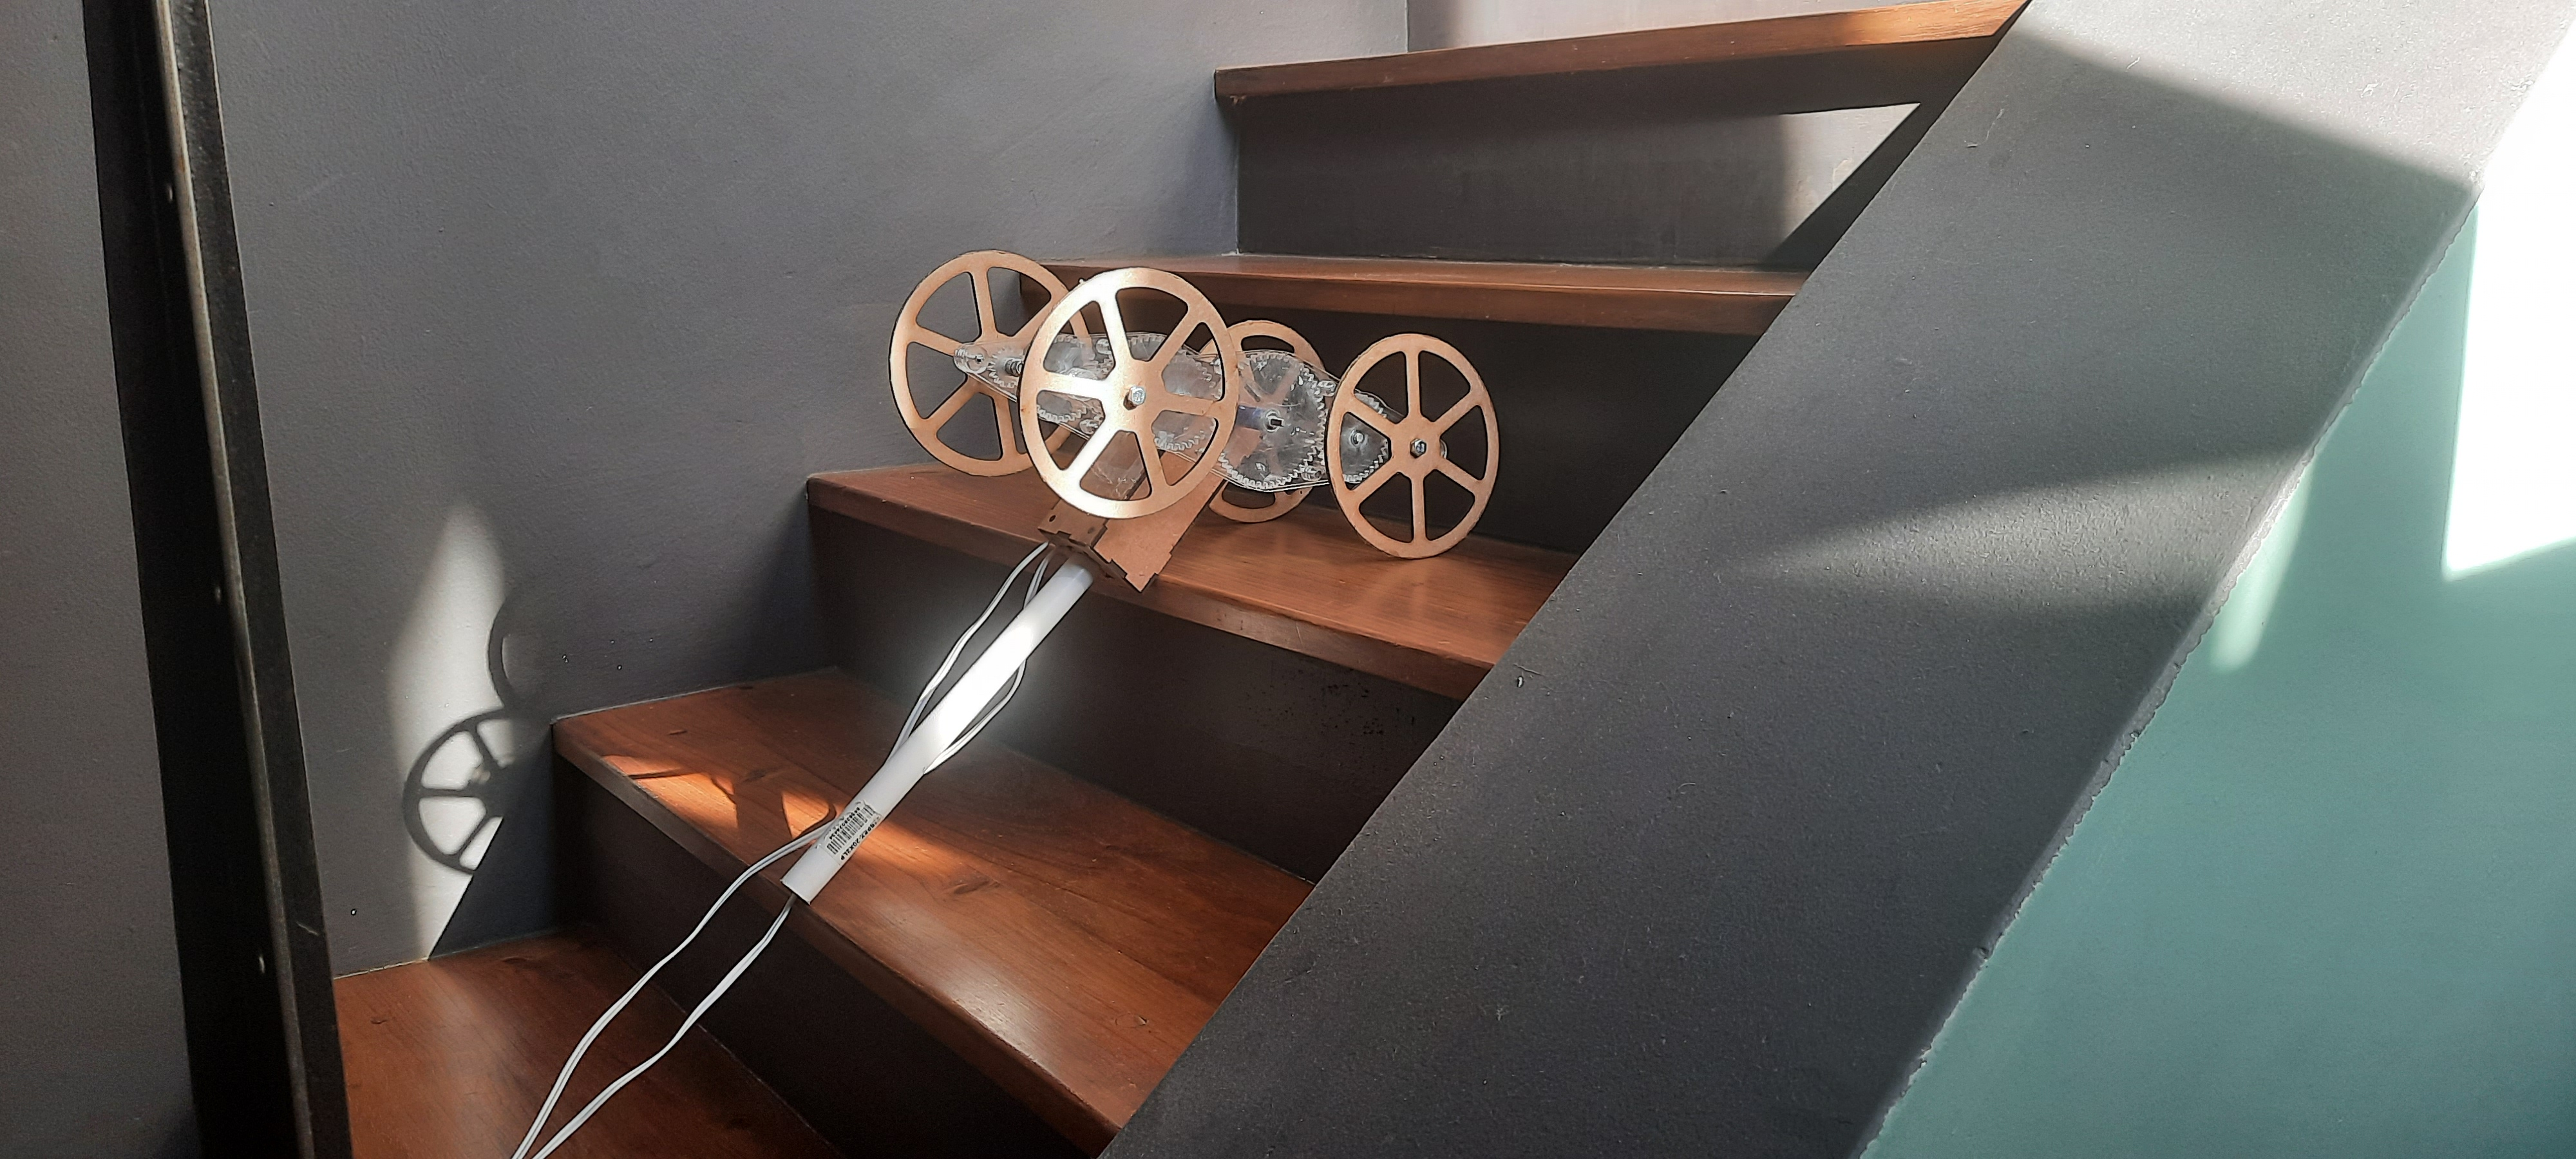
\includegraphics[width=0.8\textwidth]{device-climbing}
	\caption{Device climbing stairs.}
	\label{fig:device-climbing}
\end{figure}
%When the motor is turning it also acts as a generator, and produces a voltage known as back emf which is proportional to the speed of the motor. 
%\begin{equation}
%	E_b \propto \omega
%\end{equation}
%Where $E_b$ is the back emf and $\omega$ is the speed of the motor.
%
%The approximate circuit diagram of a DC motor is shown in figure ???. The current running through the motor is proportional to the difference between the supply voltage and the back emf.
%\begin{subequations}
%	\begin{align}
%	I &= \frac{V-E_b}{R_a
%	I &\propto V-E_b
%	\end{align}
%\end{subequations}